%-------------------------------- Configurações --------------------------------

\documentclass[a4paper,         % Tamanho do papel: A4
	           abntfigtabnum,
	           noindentfirst,
	           normaltoc,
	           pnumplain,
	           notimes,
	           sumariocompleto,
%	           capchap,
]{abnt}

\usepackage[utf8]{inputenc}
\usepackage[T1]{fontenc}
\usepackage[brazil]{babel}
\usepackage{graphicx}
\usepackage[pdfborder={0 0 0}]{hyperref} % http://www.tug.org/applications/hyperref/manual.html
\usepackage[alf,bibjustif]{abntcite}
\usepackage{listings2} % http://www.atscire.de/index.php?nav=products/listings2
\usepackage{textcomp}
\usepackage[usenames,dvipsnames]{color} % http://en.wikibooks.org/wiki/LaTeX/Colors
\usepackage{amsmath}
\usepackage{lscape}

%-------------------------------- Highligthing de código ---------------------------------

\lstset{
    basicstyle=\ttfamily,
    breaklines=true,
    language=Java,
    columns=flexible,
    numberbychapter=false,
    captionpos=b,
    showstringspaces=false,
    stringstyle=\color{red}\textit,
    keywordstyle=\color{blue}\textbf,
    emphstyle=\color{magenta}\textbf,
    numbers=none,
    numberstyle=\ttfamily\footnotesize,
    stepnumber=1,
    numbersep=10pt,
    keywords={class, for, while, if, else, and, or, break, continue, return, assert, import, do, true, false, try, catch, throws, private, public, void, int, float, double, byte, short, char, new},
    emph={ABSTRACT,MESH_TERMS,PMID,TITLE,AUTHOR_NAMES,JOURNAL_TITLE,PUB_YEAR,AUTHOR_KWS,AUTHOR},
    emph={[2]Funcionalidade, Como, Eu, E, quero, Para, Cenario, Dado, Quando, Entao, should, should_not, @matcher, context, it, describe, expect, to, world, @step, step, assert_equal, fail, expect, to_not, raise_error},
    emphstyle=[2]\color{MidnightBlue}\textbf,
    frame=none,
}
\renewcommand{\lstlistingname}{Listagem}


%--------------------------------- Informações ---------------------------------

\titulo{BioSearch Refinement: Um sistema para facilitar a busca de artigos relevantes no PubMed}
\autor{Kirill Lassounski}
\instituicao{Universidade Estadual do Norte Fluminense Darcy Ribeiro}
\orientador[Orientadora: ]{Sahudy Montenegro González}
\coorientador[Co-orientadora:]{Annabell Del Real Tamariz}
\comentario{Monografia apresentada junto ao Curso de Graduação em Ciência da
Computação da Universidade Estadual do Norte Fluminense Darcy Ribeiro como
requisito para obtenção do título de Bacharel em Ciência da Computação, sob
orientação da Prof. Dra. Sahudy Montenegro González e Prof. Dra. Annabell Del Real Tamariz}
\local{Campos dos Goytacazes/RJ}
\data{2012}




%--------------------------------- Documento -----------------------------------

\begin{document}
    
    
    
    \capa
    \folhaderosto
    
    \begin{titlepage}
\begin{folhadeaprovacao}
    Monografia sob o título \textit{BioSearch Refinement: Um sistema para facilitar a busca de artigos relevantes no PubMed}, defendida por Kirill Lassounski e aprovada no dia dd/mm/yyyy, em Campos dos Goytacazes, Estado do Rio de Janeiro, pela banca examinadora constituída pelos doutores:
    \setlength{\ABNTsignthickness}{0.4pt}
    \setlength{\ABNTsignskip}{2cm}

    \assinatura{Prof. Dra. Annabell Del Real Tamariz \\ Orientador}
    \assinatura{Prof. Dr. Luis Antonio Rivera Escriba \\ Universidade Estadual do Norte Fluminense de Darcy Ribeiro}
    \assinatura{Prof. Dr. Jorge \\ Universidade Estadual do Norte Fluminense de Darcy Ribeiro}
\end{folhadeaprovacao}
\end{titlepage}
   
    \begin{titlepage}
 \vspace*{5cm}
 \begin{flushright}
  "Por pensarem ansiosamente no futuro, esquecem o presente, de tal forma que acabam por nem viver no presente nem no futuro. Vivem como se nunca fossem morrer e morrem como se nunca tivessem vivido."\\\textit{Buda Sidarta Gautama}
  \vspace{1cm}
 \end{flushright}
 
 \vspace*{5cm}
 \begin{flushright}
  "Um homem não pode fazer o certo numa área da vida, enquanto está ocupado em fazer o errado em outra. A vida é um todo indivisível."\\\textit{Mahatma Gandhi}
  \vspace{1cm}
 \end{flushright} 
\end{titlepage}




    \begin{titlepage}
\begin{center}
\textbf{AGRADECIMENTOS} \\ [2.5cm]
\end{center}
Agradeço a UENF, por me abrigar e proporcionar os meios para o aprendizado. Às minhas professoras, amigas e orientadoras Sahudy e Annabell por me ensinarem à pesquisar, estudar e computar. E a Elena e Camila por me apoiarem e ter me motivado a ser sempre melhor. Obrigado.
\end{titlepage}




    
    
    \sumario
    \listoffigures
    \listoftables
    \begin{resumo}
A quantidade de informação na \emph{Internet} está em constante crescimento, o que demanda técnicas modernas de recuperação de informação para organizá-la. O NCBI é um portal de informação biomédica e possui em sua estrutura o banco de dados PubMed que contém artigos científicos de jornais e revistas e outros recursos. O objetivo do \emph{BioSearch Refinement} é ajudar o pesquisador a encontrar informação relevante com mais facilidade e rapidez no banco de dados PubMed. O sistema permite a sumarização dos artigos através da representação de seus principais conceitos utilizando palavras-chave, e estas palavras podem ser usadas para refinar o conjunto de artigos exibidos. Neste trabalho também é apresentado o PubMed Dataset que provê o acesso ao NCBI e permite a criação de conjuntos de dados para teste com os dados do PubMed.
\end{resumo}

\begin{abstract}
The amount of information on the Internet is at constant growth and it demands modern information retrieval techniques to organize it. The NCBI is a biomedic information portal, having in its structure the PubMed database that contains scientific articles and other resources. The BioSearch Refinement goal is to help researchers to find relevant information on PubMed easily and quickly. The system provides article summarization through the representation of its basic concepts using keywords, these keywords can be used to refine the set of articles displayed on the interface. This paper also presents the PubMed Dataset that provides access to NCBI and allows the creation of data sets using PubMed articles to test informaton retrieval systems.
\end{abstract}


    \chapter{Introdução}
A capacidade de visualizar as informações de maneira clara e organizada, é importante para qualquer usuário. Geralmente, as informações com as quais se lida no dia-a-dia são textuais e necessitam de tempo para serem interpretadas. Quando a quantidade destes dados é grande, se leva um tempo considerável para encontrar a informação de relevância. Nas décadas de 50, a informação começou a migrar do papel para os dispositivos eletrônicos, onde pode ser mais facilmente armazenada, conservada e organizada. O crescimento da quantidade de documentos armazenados tornou difícil a recuperação daqueles que são de interesse em um dado momento. A recuperação de informação é uma área da ciência da computação que lida com a armazenamento, organização, representação e acesso à itens de informação \cite{Yates1999}.

O tráfego na Internet tem crescido numa escala de 100\% a cada ano a partir da década de 90. Atualmente esta taxa diminuiu e está em 50\% \cite{Odlyzko2003}. A previsão é de que esta taxa diminua para 35\% no período até 2013 \cite{Cisco2009}. Apesar da diminuição da taxa de crescimento do tráfego na Internet, a quantidade de informações sendo lidas e armazenadas na grande rede cresce diariamente e a capacidade de extrair conhecimento relevante se torna uma dificuldade. Muitas vezes a informação está acessível, mas os métodos de busca atuais tornam difícil o seu acesso.

A crescente massa de informação criou a necessidade da concentração desta em um lugar em comum onde a informação possa ser visualizada, organizada e classificada. Existem diversos bancos de dados e bibliotecas que disponibilizam informação, seja ela científica ou tecnológica. Como exemplos pode-se destacar:
\begin{itemize}
    \item PubMed\footnote{\href{http://www.ncbi.nlm.nih.gov/pubmed}{http://www.ncbi.nlm.nih.gov/pubmed}}:
    possui mais de 21 milhões de citações de literatura biomédica do MEDLINE, periódicos científicos e e-books.
    \item Science Direct\footnote{\href{http://www.sciencedirect.com/}{http://www.sciencedirect.com/}}:
    banco de dados do SciVerse com mais de 10 milhões de artigos científicos e capítulos de livros.
    \item CiteULike\footnote{\href{http://www.citeulike.org/}{http://www.citeulike.org/}}:
    serviço gratuito para encontrar e gerenciar referências acadêmicas, possui atualmente cerca de 5 milhões de documentos.
    \item IEEE Xplore\footnote{\href{http://ieeexplore.ieee.org/Xplore/guesthome.jsp}{http://ieeexplore.ieee.org/Xplore/guesthome.jsp}}:
    possuindo 3 milhões de documentos, o portal da IEEE provê acesso à informação técnica em engenharia e tecnologia.
    \item ACM Digital Library\footnote{\href{http://dl.acm.org/}{http://dl.acm.org/}}:
    coleção de artigos e registros bibliográficos sobre os campos de computação e tecnologia da informação.
\end{itemize}

Independente do mecanismo de busca, se a base de dados for muito grande, o que acontece em muitos casos, serão retornadas grandes quantidades de documentos que tornam tedioso o processo de busca no conjunto de resultados. Quando esta quantidade de resultados ultrapassa centenas de itens, o processo de busca se torna cansativo mesmo fazendo uma leitura dinâmica nos resultados. Os sistemas de recomendação sugerem documentos relevantes baseado em informações providas por outros usuários de um sistema, gerando uma melhora no processo de busca \cite{Jannach2010}, mas este tipo de algoritmo não reflete na quantidade de documentos retornados. O PubMed utiliza um sistema de recomendação no campo "\emph{Related searches}", que disponibiliza frases de busca relacionadas com a submetida pelo usuário.

Para reduzir a quantidade de documentos disponibilizados em uma busca, pode-se dividi-los em categorias rotuladas por palavras-chave. Cada palavra-chave representa uma porção do total de documentos exibidos e representa um tema ou assunto abordado pelos documentos do sub-conjunto. A extração de palavras-chave é uma técnica que obtém termos descritores a partir dos textos de documentos, que podem ser usados para indexar/recuperar ou sumarizar os dados documentos.

Neste trabalho é apresentada uma abordagem de extração de palavras-chave a partir de documentos, e além disso é apresentada uma maneira de utilizar estas palavras para resumir sub-conjuntos destes documentos. Para avaliar os resultados obtidos foi criada uma biblioteca de construção de conjuntos de dados de teste obtidos do PubMed.

\section{Formulação do problema}
A grande massa de informação disponível criou a necessidade de mecanismos que possam organizá-la de maneira clara para os usuários. Esta dificuldade não é restrita à Internet, mas também existe em grandes empresas e instituições. Como uma grande parte desta informação está na forma de texto, muito esforço tem sido feito nas comunidades de recuperação de informação para melhorar os algoritmos de indexação/ordenação de documentos.

Como um exemplo pode-se destacar o \emph{National Center for Biotechnology Information} (NCBI), que provê informações científicas sobre biomedicina e genomas. É um  portal mantido pelo governo dos Estados Unidos da América utilizado por pesquisadores de todas partes do mundo servindo informações em seus estudos. Um de seus bancos de dados mais acessado é o PubMed, que guarda cerca de 21 milhões de artigos científicos na área de saúde, um número que cresce continuamente. Os resultados exibidos pelo PubMed formam um lista linear de artigos científicos que não possibilitam o usuário de ter um panorama dos tópicos sendo abordados por estes artigos ou de refinar os artigos até atingir uma necessidade em particular. Esta grande quantidade de informação gera dificuldade no processo de localização do material desejado com os métodos de busca tradicionais.

O processo de busca no portal se utiliza do modelo booleano\footnote{\href{http://www.nlm.nih.gov/pubs/techbull/ja97/ja97\_pubmed.html}{http://www.nlm.nih.gov/pubs/techbull/ja97/ja97\_pubmed.html}} onde o usuário especifica palavras-chave e as conecta utilizando operadores booleanos (\emph{AND,OR} e \emph{NOT}). As palavras-chave podem ser buscadas em diversos atributos de um documento como autor, ano de publicação, termos MeSH, resumo, título entre outros. 

Neste tipo de busca, os documentos retornados são filtrados de acordo com os termos que estão contidos nele e os que não estão contidos. Este tipo de busca é conhecido por retornar grandes conjuntos de resultados, além de possuir uma complicada lógica de formulação das buscas, logo um usuário inexperiente muitas vezes tem dificuldade em efetuar buscas satisfatórias \cite{Jackson2007}. 

Neste cenário, a quantidade de artigos retornados em uma busca geralmente é muito extensa e para diminuir o número de resultados o usuário se vê obrigado a inserir mais termos para refinar sua busca. Para exemplificar o problema, ao se fazer uma busca no PubMed com um termo de busca bem geral como \emph{“tuberculosis”}, foram retornados 192.499 artigos. Ao se especificar este termo para \emph{“human [Title/Abstract] AND mycobacterium tuberculosis [Mesh]”} a quantidade de resultados diminuiu para 3.084, mas ainda assim permanece grande para uma leitura rápida e o pesquisador se vê obrigado a especificar mais a sua busca. Como observado por \cite{Perez-Iratxeta2001}, em uma busca exploratória, onde o pesquisador seleciona termos de seu conhecimento para melhorar os resultados da busca, muitas vezes não se tem conhecimento de um determinado termo até que este seja identificado no texto.

\section{Objetivos}
Como objetivo principal, se propõe um método de refinamento de artigos do banco de dados PubMed através da utilização de palavras-chave. Cada palavra-chave representa um tema que é amplamente abordado por artigos retornados de uma busca ao banco. O método proposto permitirá o(a) pesquisador(a) encontrar com mais facilidade e rapidez artigos relevantes no PubMed. O objetivo secundário é a construção de uma \emph{interface} que melhore a navegação e visualização dos artigos.

Para atingir tal objetivo foi desenvolvido o sistema BioSearch Refinement, uma aplicação que pode sumarizar e dar uma visão geral dos artigos retornados em uma busca. Para destacar os temas sendo mais abordados em uma determinada busca são utilizadas palavras-chave. As palavras-chave podem ajudar o leitor a decidir se um determinado documento é de seu interesse ou não. Elas dão uma breve descrição sobre o conteúdo mais importante sendo abordado, mas muitas vezes os documentos não possuem palavras-chave e o processo de atribuição é muito custoso \cite{Lui2007}. Além da sumarização, palavras-chave podem ser usadas para indexar documentos e também para tornar uma busca mais precisa \cite{Turney1999}. Neste trabalho usamos as palavras-chave para fazer sumarização de grupos de documentos, onde cada palavra-chave representa uma parte deste grupo. Com estas palavras pode-se reduzir a quantidade de resultados retornados facilitando o processo de busca.

A ideia central do algoritmo é extrair  conceitos a partir dos resumos dos artigos, que serão utilizados para determinar quais artigos são referenciados por um determinado conceito. Os conceitos que referenciarem um maior número de artigos serão considerados mais generalistas e serão escolhidos como palavras-chave que sumarizam os principais assuntos de uma busca. A extração se utiliza de técnicas de processamento de linguagem natural e frequência de termos para determinar os conceitos. O algoritmo é aplicado no sistema BioSearch Refinement que é um sistema com o propósito de simplificar e ajudar o pesquisador a encontrar material relevante.

\section{Organização}
No capítulo 2 são apresentados os trabalhos relacionados e as metodologias usadas para a sumarização de documentos e extração de palavras-chave. Também são introduzidos os conceitos da recuperação de informação necessários para compreender o capítulo 3. No capítulo 3 é apresentado o sistema \emph{BioSearch Refinement} e as partes que o compõem, o \emph{Extraction Engine} e o \emph{PubMed Dataset}. O capítulo 4  apresenta os resultados obtidos para as partes que compõem o sistema e também discute estes resultados. No capítulo 5 são tiradas as conclusões sobre o trabalho feito como também são apresentadas as contribuições e possíveis trabalhos futuros.


    \chapter{Recuperação de informação}
Um sistema que recupera informação permite um usuário manusear a informação contida em documentos, que na maioria das vezes estão em formato de texto. O objetivo do sistema é ajudar a encontrar a informação indicando a sua localização, ou informar se ela de fato existe no domínio buscado. O resultado da recuperação é um conjunto de documentos, dos quais alguns são uteis para o usuário (relevantes) e outros não (irrelevantes). Basicamente um sistema de recuperação possui: uma forma de representar os documentos, uma forma de representar a necessidade do usuário e a comparação entre as duas representações \cite{Goker2009}. 

As palavras-chave são unidades textuais que servem para representar documentos, elas possuem a essência do documento, descrevendo de maneira clara e precisa o seu conteúdo. Neste trabalho palavras-chave representam tanto termos simples \emph{“influenza”} como termos compostos (\emph{keyphrases}) \emph{“influenza h1n1 virus”}. Os termos compostos são mais valorizados, pois são considerados como sendo mais informativos para descrever um documento \cite{Fagan1989}.

Para determinar os temas principais sendo abordados em um conjunto de documentos, é preciso identificar cada documento com um conjunto de um ou mais descritores que reflitam os temas principais sendo abordados, tarefa da indexação automática.

\section{Indexação automática}
A indexação automática associa termos descritivos aos documentos de um conjunto através do programa de computador, no intuito de permitir a eficiente recuperação e armazenamento destes em um sistema informatizado \cite{Gonzalez2006}. O início da indexação automática se deu nos anos 50, naquela época a quantidade de informação guardada em computadores era limitada, logo não eram necessárias técnicas muito avançadas para organizá-la. Basicamente cada documento era indexado manualmente com alguns termos que o descreviam, e quando o usuário fazia um busca, os termos da busca eram comparados com os termos do documento e exibidos aqueles documentos que satisfaziam a igualdade de termos de busca para termos descritores. Mas a rotulação manual de cada documento exige um profissional especializado com conhecimento do domínio deste documento e tempo para identificar os descritores e provavelmente a quantidade de pessoal especializado em indexação de documentos não é suficiente para indexar com qualidade a crescente massa de documentos que vem surgindo.

Uma ótima análise do processo de obtenção de descritores foi feita por Gonzalez et al. \cite{Gonzalez2006} e a seguir são abordados os seus principais pontos. Nem todos os termos existentes em um texto podem ser considerados descritivos, por isso existem diversas técnicas e abordagens para a obtenção de descritores para um documento. Mas quase todas as abordagens possuem uma fase em comum, a fase de pré processamento do texto. Nesta fase, o texto é preparado para a obtenção dos descritores, e suas operações estão de acordo com a abordagem sendo adotada.

 Geralmente o texto passa pela tokenização (identificação dos itens léxicos do texto), seleção dos descritores e conflação \cite{Yates1999}. Se a abordagem utilizada se utiliza de informações linguísticas, técnicas de processamento de linguagem natural podem ser usadas para determinar as relações morfo-sintáticas entre as palavras. Estas relações são obtidas através do \emph{part-of-speech tagging}, explicado adiante.

Na fase de seleção de descritores ocorre a eliminação de \emph{stopwords}, que elimina palavras pouco representativas como preposições, artigos e conjunções. A eliminação destas palavras diminui a quantidade de possíveis descritores ganhando economia, mas por outro lado diminui a representatividade. Uma maneira de aproveitar estas palavras é apenas permiti-las como ligação entre palavras relevantes na análise morfo-sintática, gerando assim descritores mais representativos. Vale ressaltar que em alguns domínios existem palavras que podem ser consideradas \emph{stopwords}, mas em outros domínio não são. Um exemplo disso são palavras como remédio, doença, paciente, resultado e análise no domínio da medicina. Palavras assim tem pouco valor de indexação e recuperação, pois a maior parte dos documentos possui estes termos.

Uma técnica muito utilizada para a representação de termos similares como sendo um só é a normalização, onde palavras com variações linguísticas são interpretadas como sendo a mesma palavra ou conceito. Utilizando a normalização, o cálculo de frequência pode ser ampliado para um determinado termo através da similaridade com outros termos do texto. A forma de normalização que é usada neste trabalho, é a conflação. Segundo \cite{Gonzalez2006} as formas de conflação mais usadas é o \emph{stemming} e a lematização. Um algoritmo de \emph{stemming} ou em português, radicalização, trunca as palavras para deixar apenas o radical desta palavra, permitindo assim remover plurais e sufixos que causam a variação de uma mesma palavra. Já a lematização reduz a palavra até sua forma canônica: \emph{lemma}(working) = work ; \emph{lemma}(worked) = work. A lematização possui resultados melhores, porém é mais difícil de ser aplicada, já que em alguns casos é necessário o uso de um dicionário para poder determinar o lema corretamente: \emph{lemma}(better) = good.

Como mostrado no livro de \cite{Moens2000}, na indexação automática a seleção de descritores pode ser subdividida em duas abordagens. Na primeira, os termos são extraídos diretamente do texto através de um processo de filtragem afim de deixar apenas os termos mais descritivos. Na segunda abordagem, os termos são selecionados de um vocabulário controlado (\emph{thesaurus}), ou seja, atribuídos aos documentos. Um \emph{thesaurus} difere de um dicionário pelo fato de possuir relações entre palavras e sinônimos ao invés de definições, fornecendo assim agrupamentos de palavras com mesmo significado.
 
\subsection{Extração de palavras-chave}
A extração de termos não se baseia no uso de um vocabulário controlado para a seleção das palavras-chave para um documento, em vez disso, utiliza termos do próprio texto. Pode trabalhar usando abordagens léxicas, estatísticas ou híbridas para extrair descritores do texto de um documento.

A abordagem léxica segue uma sequencia de passos pré definidos para a extração dos descritores de um texto:
\begin{enumerate}
    \item Análise léxica: nesta fase são determinadas as classes gramaticais de cada palavra de um frase, com estas informações pode-se decidir quais palavras podem ser importantes ou não. Um \emph{part-of-speech tagger} (POST) serve para fazer uma rotulação das palavras que compõem o texto, onde cada rótulo representa a classe gramatical de uma palavra.
    \item Análise sintática: esta análise serve para gerar descritores compostos por mais de uma palavra, os descritores são criados baseado em padrões sintáticos definidos previamente. Uma máquina de estado é alimentada com os rótulos e trunca a frase em termos candidatos(\emph{chunking}).Geralmente os padrões sintáticos são montados para selecionar palavras-chave compostas por substantivos (\emph{noun chunking}), pois o substantivo é a classe gramatical que nomeia objetos, pessoas, substâncias, lugares e serve para identificar sobre o que se está discursando \cite{Gucker1966}.
\end{enumerate}
De todos os termos resultantes do processo de \emph{chunking} são selecionados os melhores descritores usando-se de alguma metodologia específica. Geralmente são calculados pesos para cada termo candidato e são selecionados aqueles que possuem maior peso.

As técnicas estatísticas fazem cálculos para determinar a relevância de um termo em um texto e então decidir quais destes termos identificarão o documento. Alguns sistemas trabalham as relações de termos no conjunto de documentos total (\emph{corpus}) e outros se utilizam apenas do domínio de um documento, mas o que todos estes sistemas tem em comum é a utilização de \emph{corpus} de treinamento para criar modelos de predição que determinam se um termo é ou não relevante. \cite{Berry2010} afirmam que os sistemas que se utilizam de métodos orientados a \emph{corpus} geralmente trabalham com unigramas (palavra-chave de apenas uma palavra) o que limita a qualidade dos descritores por serem usados em múltiplos e diferentes contextos.

Em uma abordagem híbrida são usadas ambas as técnicas citadas anteriormente buscando aproveitar as melhores qualidades de cada uma para se determinar descritores com uma maior qualidade. Neste trabalho utilizamos esta abordagem, primeiramente determinamos os possíveis descritores de um documento através da obtenção das classes gramaticais das palavras do texto utilizando o POST e em seguida extraímos \emph{noun chunks} utilizando padrões sintáticos. Para determinar quais destes termos são relevantes é utilizado um novo algoritmo que descobre a relação entre os termos candidatos fazendo um cruzamento de informações e determina as palavras-chave através de um peso que envolve a frequência de termos e o número de palavras que compõem uma palavra-chave.

\subsubsection{Part of speech tagger (rotulador)}
Para o processamento de linguagem natural utiliza-se a API LingPipe\footnote{\href{http://alias-i.com/lingpipe/}{http://alias-i.com/lingpipe/}} da Alias-i sob a licença \emph{Alias-i ROYALTY FREE LICENSE VERSION 1}. Uma API (\emph{Application Programming Interface}), também chamada de biblioteca, é um conjunto de códigos de uma determinada linguagem de programação que permitem ao utilizador desta, acelerar o seu processo de desenvolvimento através da reutilização destes códigos. Neste caso, a funcionalidade essencial é o rotulamento, que é implementado pela API utilizando HMM (\emph{Hidden Markov Model}, uma máquina de estados finitos. Foi mostrado que as cadeias de Markov são muito eficientes na extração de informação quando se trata de informação sensível ao contexto como texto em linguagem natural oferecendo equilíbrio entre simplicidade e expressividade de contexto\cite{Freitag2000}. As cadeias de Markov determinam a probabilidade da classe gramatical de uma palavra baseado na classe gramatical de outras palavras da frase.

Como todo modelo estatístico, o rotulador necessita de um \emph{corpus} para ser treinado e neste caso é usado o MEDLINE corpus já que o domínio de linguagem é biomédico. Rotuladores desenvolvidos para textos gerais não funcionam bem quando aplicados ao MEDLINE. O rotulador de Brill \cite{Brill1992} aplicado a 1000 frases selecionadas aleatoriamente do MEDLINE, obteve uma exatidão de 86.8\% usando o conjunto de rótulos de \emph{Penn Treebank}. Esta baixa performance esta relacionada à especificidade do vocabulário do MEDLINE. O rotulador MedPost \cite{Smith2004} foi desenvolvido para satisfazer a necessidade de uma alta precisão no rotulamento treinado sobre o MEDLINE corpus. No teste de 1000 frases, ele obtêm exatidão de 97.43\% usando o conjunto de rótulos nativo.

\subsection{Atribuição de palavras-chave}
O método de atribuição de termos seleciona os descritores de um vocabulário controlado que melhor descrevem um documento. Uma maneira muito utilizada atualmente para a representação de domínios se chama ontologia, onde palavras-chave são utilizadas para representar conceitos.

\subsubsection{Ontologias}

 Segundo Gruber \cite{Gruber1993} uma ontologia é a especificação de um vocabulário para uma determinado domínio, definição de classe, relações, funções e outros objetos. Ela descreve formalmente um domínio e é composta por termos e o relacionamento entre estes \cite{Antoniou2004}. As ontologias são muito utilizadas nos campos de biologia e medicina, pois estas possuem uma grande quantidade de termos e relações entre eles. Tem sido feito muito esforço nas comunidades acadêmicas de vários países na pesquisa e desenvolvimento desta tecnologia. As principais ontologias na área de biomedicina atualmente são a \emph{Gene Ontology} (GO) \cite{GO2000} que faz um mapeamento semântico de genes e produtos genéticos como proteínas, \emph{Medical Subject Headings} (MeSH) \cite{MESH2000} utilizado pelo NCBI na indexação de documentos científicos e a \emph{Foundational Model of Anatomy}  (FMA) \cite{FMA2003} que é uma ontologia para representação de anatomia humana.

\section{Sistemas de refinamento}

A seguir são apresentados alguns trabalhos de sistemas que permitem a categorização de artigos retornados a partir de uma busca do PubMed. Como se pode perceber existem diversas abordagens para o agrupamento de artigos similares, mas poucos dos trabalhos pesquisados fazem a utilização de um algoritmo próprio de extração de palavras-chave para classificar documentos. \cite{Maron1958} tiveram a ideia de organizar os documentos baseando-se em uma probabilidade de relevância. Os termos de busca inseridos pelo usuário eram processados pelo teorema de Bayes e era determinada a probabilidade de cada documento ser relevante para o usuário. A vantagem desta abordagem era eliminar a busca booleana que é ineficiente quanto à seleção de documentos relevantes.

\subsection{GoPubMed}

Uma ferramenta que utiliza uma abordagem baseada em ontologias para organização dos resultados obtidos do PubMed é o GoPubMed\footnote{\href{http://www.gopubmed.com}{http://www.gopubmed.com}} \cite{Doms2005}, que utiliza o Gene Ontology e o MeSH. Este sistema divide as informações em quatro categorias principais (o que, quem, onde e quando) através das informações obtidas do PubMed e  permite o usuário restringir sua busca utilizando estes campos.

\begin{enumerate}
\item A categoria "o que", é processada utilizando-se dos resumos retornados a partir de uma busca à base de dados do PubMed e através de ontologias o sistema cria um árvore onde cada nível representa um tópico sendo abordado pelos artigos da pesquisa. O uso de ontologias permite a descrição de termos que são identificados na ontologia, descrevendo sinônimos e mostrando uma árvore de relacionamentos.

\item Na categoria "quem", os artigos podem ser filtrados por autores e centros. Nesta categoria podem ser visualizados os dados das instituições e cientistas. O sistema leva em conta que um determinado autor publica sobre temas similares, com os mesmo co-autores e nas mesmas revistas, estas associações são mapeadas em uma rede semântica que determina a probabilidade de dois artigos serem escritos pela mesma pessoa.

\item Em "onde", estão disponibilizadas as localizações de pessoas, universidades e centros de pesquisa, além disso são listadas também as melhores revistas (com alto fator de impacto).

\item A categoria "quando", mostra os anos das publicações e permite selecionar a data de publicação para reduzir o número de artigos sendo exibidos.
\end{enumerate}

Neste trabalho não optamos pela utilização de ontologias, pois o vocabulário destas é controlado e deve ser constantemente atualizado. Alguns artigos não possuem termos MeSH por serem inovadores ou antigos. As palavras-chave retiradas diretamente do resumo e título são mais representativas e mais descritivas para um determinado artigo do que termos predefinidos.

\subsection{XplorMed}
A ferramenta XplorMed de \cite{Perez-Iratxeta2001} é uma das primeiras a propor uma maneira de melhorar a busca por artigos relevantes no PubMed e se utiliza de cálculos aritméticos simples para criar relacionamentos entre palavras nos resumos e, assim, identificar palavras-chave. Neste sistema, a relação entre palavras é criada utilizando lógica fuzzy onde há um relacionamento entre duas palavras \emph{x} e \emph{y} medido por um valor entre 0 e 1. O valor é medido pela seguinte equação:

\begin{centering}
\textbf{
núm. de resumos que contém \emph{x} e \emph{y} / núm. total de resumos que contém \emph{x} ou \emph{y}
}
\end{centering}

O grau de inclusão mostra que palavras mais gerais incluem palavras mais especificas, a inclusão de \emph{x} em \emph{y} é:

\begin{centering}
\textbf{
núm. de resumos que contém \emph{x} e \emph{y} / núm. total de resumos que contém \emph{x}
}
\end{centering}

Palavras importantes são aquelas que possuem um alto valor associativo, valor que é calculado pelo somatório do grau de inclusão de todas as palavras que são relacionadas à palavra em questão. O problema desta abordagem é que ela restringe o relacionamento entre palavras a apenas duas palavras. O usuário do sistema pode restringir sua busca navegando pelos relacionamentos das palavras geradas e assim reduzir o número de artigos sendo exibidos. Também, é possível visualizar as frases que possuem uma determinada relação. O processo é iterativo e pode gerar uma cadeia de palavras, ou seja, a cada redução do conjunto de resultados é feita uma nova análise do relacionamento entre as palavras.

Para avaliar a capacidade de melhorar a precisão de resultados efetuados no PubMed, foram selecionadas 4 revisões. Foram selecionadas cuidadosamente palavras-chave que representassem a revisão e foi feita uma busca no PubMed, a precisão foi calculada com os artigos retornados pelo PubMed e os artigos contidos na revisão sendo analisada. Utilizando uma cadeia de palavras-chaves geradas pelo XplorMed se chegou à uma precisão mais elevada (0.034 -> 0.092 em um dos artigos). A precisão é a divisão do número de documentos relevantes pelo número total de documentos retornados.

\subsection{Anne O`Tate}
Um trabalho similar com o que está sendo proposto é o Anne O`Tate, publicado por \cite{Smalheiser2008}. Neste trabalho é descrita uma aplicação que facilita o processo de busca e navegação para um usuário do PubMed. Os artigos podem ser analisados sob diversos pontos de vista, como por exemplo palavras mais importantes de resumo e títulos, tópicos e autores. Ao clicar em um destes itens, os artigos são filtrados e exibidos aqueles que satisfazem as condições dos filtros selecionados. Também é implementado um algoritmo de agrupamento de artigos por categorias que permite a distribuição de artigos em tópicos em comum.

Os termos extraídos dos artigos do PubMed são guardados em um banco de dados e são atribuídos às categorias semânticas do \emph{Unified Medical Language System}(UMLS) através do programa \emph{MetaMap}\footnote{\href{http://metamap.nlm.nih.gov/}{http://metamap.nlm.nih.gov/}} do \emph{National Library of Medicine} (NLM). Este programa faz o mapeamento de textos da área de biomedicina para um tesauro do UMLS que  possui categorias pré-definidas. Estas categorias são usadas como palavras-chave para referenciar os assuntos principais sendo abordados em um artigo. Os artigos exibidos pelo Anne O`Tate podem ser filtrados através destas categorias.

Outra funcionalidade interessante é a expansão de literatura que ocorre quando o número de artigos sendo exibidos para o usuário é menor do que cinquenta. O sistema busca artigos com temas similares utilizando o sistema de artigos relacionados do PubMed. Os artigos relacionados são selecionados apenas se forem relacionados com mais de 40\% dos artigos originais.

Para dar uma visão geral dos artigos retornados a partir de uma busca, é utilizada a função de categorização por tópicos. Esta função utiliza os termos MeSH para dividir os artigos em áreas afins. Artigos recentes e antigos não possuem termos MeSH e são colocados em categorias "Muito recentes" e "Não indexados" respectivamente, os outros artigos são categorizados em não mais do que 15 categorias MeSH utilizando um algoritmo de agrupamento.

A ferramenta Anne O`Tate implementa diversas funcionalidades interessantes como agrupamento de artigos por tópicos e organização por autores e ano, dando a possibilidade do pesquisador encontrar material relevante sem a necessidade de modificar o termo de busca do PubMed. Fato notável é que esta ferramenta tem a capacidade de processar até 25.000 artigos e distribuí-los em categorias em um tempo aceitável para um sistema \emph{Web}.

A maioria dos sistemas que foram estudados utilizam-se dos dados do PubMed para fazer o agrupamento de artigos em sub-tópicos, a utilização de campos como datas de publicação, autores e localidades são óbvias. A divergência entre estes sistemas está relacionada às técnicas e os algoritmos usados para determinar os sub-domínios em grupos de artigos retornados a partir do PubMed. Muitos dos sistemas utilizam-se de ontologias para atribuir descritores aos artigos como o GoPubMed \cite{Doms2005}, PubReMiner \footnote{\href{http://bioinfo.amc.uva.nl/human-genetics/pubreminer/}{http://bioinfo.amc.uva.nl/human-genetics/pubreminer/}} e PubMedAssistant \cite{Ding2006}, sistemas como os de  XplorMed \cite{Perez-Iratxeta2001} e BioIE \cite{Divoli2005} extraem relacionamentos entre as palavras contidas em resumos e títulos para representar e agrupar artigos similares e ainda existem sistemas que mostram artigos relacionados e artigos ordenados por relevância como em HubMed \cite{Eaton2006} e Relemed \cite{Siadaty2007} respectivamente.

O sistema apresentando neste trabalho utiliza uma abordagem diferente para o agrupamento de artigos, através do processamento de linguagem natural são extraídos possíveis descritores para os artigos e estes por sua vez passam por um processo para detectar os mais descritivos. Essa abordagem fornece descritores independentes de vocabulários controlados como o MeSH ou GO, resultando em conceitos mais genuínos para um determinado artigo. Utilizando estes conceitos extraídos localmente, são obtidos os conceitos globais que descrevem temas em comum.

\section{Métricas de avaliação}
Para avaliar a qualidade dos resultados obtidos em um sistema de RI são utilizadas métricas que fazem comparações dos resultados obtidos por um sistema com os resultados que se esperam deste sistema. Basicamente são operações matemáticas de conjuntos que revelam valores percentuais de um determinado aspecto do sistema. As duas métricas mais conhecidas e bem aceitas na comunidade de RI são o \emph{recall} e o \emph{precision} \cite{Turpin2006}.

O \emph{recall} serve para representar a quantidade de documentos relevantes que foram recuperados, não levando em conta os documentos irrelevantes que também foram recuperados.
\\
\begin{center}
\textbf{
recall = (núm. de documentos corretamente recuperados) / (núm. total de documentos relevantes)
}
\end{center}

\emph{Precision} avalia o que o \emph{recall} não leva em conta, verificando quantos dos documentos recuperados são relevantes.
\begin{center}
\textbf{
precision = (núm. de documentos corretamente recuperados) / (núm. total de documentos recuperados)
}
\end{center}

A \emph{F1-measure} é uma métrica que expressa a média balanceada entre o \emph{recall} e o \emph{precision} \cite{Feldman2007}.
\begin{center}
\textbf{
\emph{F1-measuere} = 2 / ( (1 / \emph{recall}) + (1 / \emph{precision}))
}
\end{center}


    \chapter{BioSearch Refinement}

Para atingir o objetivo principal foi desenvolvido o sistema BioSearch Refinement, uma aplicação que pode sumarizar e dar uma visão geral dos artigos retornados em uma busca. Para destacar os temas sendo mais abordados em uma determinada busca são utilizadas palavras-chave. As palavras-chave podem ajudar o leitor a decidir se um determinado documento é de seu interesse ou não. Elas dão uma breve descrição sobre o conteúdo mais importante sendo abordado, mas muitas vezes os documentos não possuem palavras-chave e o processo de atribuição é muito custoso \cite{Lui2007}. Além da sumarização, palavras-chave podem ser usadas para indexar documentos e também para tornar uma busca mais precisa \cite{Turney1999}. Neste trabalho usamos as palavras-chave para fazer sumarização de grupos de documentos, onde cada palavra-chave representa uma parte deste grupo. Com estas palavras pode-se reduzir a quantidade de resultados retornados facilitando o processo de busca.

A ideia central do algoritmo é extrair  conceitos a partir dos resumos dos artigos, que serão utilizados para determinar quais artigos são referenciados por um determinado conceito. Os conceitos que referenciarem um maior número de artigos serão considerados mais generalistas e serão escolhidos como palavras-chave que sumarizam os principais assuntos de uma busca. A extração se utiliza de técnicas de processamento de linguagem natural e frequência de termos para determinar os conceitos.

O \emph{BioSearch Refinement} possui uma estrutura de aplicação \emph{Web} utilizando o padrão MVC (\emph{Model View Controller}), para que qualquer usuário com acesso à \emph{Internet} possa utilizar o sistema. A implementação foi feita na linguagem de programação Java, visto que ela é flexível, computacionalmente eficiente \cite{Oracle2010}, tem suporte à plataforma \emph{Web} e sendo a linguagem mais utilizada no mundo \cite{TIOBE2011}, possui uma extensa documentação e uma grande quantidade de API`s de processamento de linguagem natural. O fluxo básico de funcionamento da aplicação pode ser visto na Figura \ref{fig:1}.

\begin{figure}[h!]
    \center
    \includegraphics[scale=0.6]{imagens/processoGeralBSR.pdf}
    \caption{Processo geral do sistema \emph{BioSearch Refinement} \label{fig:1}} 
\end{figure}

O \emph{BioSearch Refinement} é composto pelo \emph{PubMed Dataset} (biblioteca de criação de conjuntos de dados explicada adiante) que se comunica com o NCBI e acessa o PubMed para obter os artigos requisitados pelo usuário. E também possui o \emph{Extraction Engine}, que é o algoritmo que determina as palavras-chave.

A interação com o sistema é dada da seguinte maneira:

\begin{enumerate}
    \item O usuário interage com aplicação fornecendo o termo de busca.
    \item O termo buscado é passado para o \emph{PubMed Dataset}  que faz a comunicação com o PubMed pela internet.
    \item Os 20 primeiros artigos mais recentes são exibidos na tela para que o usuário possa navegar. Um mecanismo de paginação é implementado, para que a aplicação seja leve e funcione com rapidez. Mais artigos poderão ser carregados se o usuário fizer uma requisição para exibir outra página.
    \item Para executar o algoritmo de extração de palavras-chave (\emph{Extraction Engine}) o usuário clica em um botão "\emph{Generate keywords}", mostrado na Figura \ref{fig:telaComBusca}.
    \item Ao finalizar o processamento, as palavras-chave mais relevantes aparecem para o usuário permitindo a filtragem dos artigos exibidos.
    \item Ao clicar em uma das palavras-chave, uma nova aba é aberta dentro da \emph{interface} do sistema. Nesta aba são exibidos os artigos relacionados com aquela palavra-chave e são geradas novas palavras-chave para aquele conjunto de artigos.
\end{enumerate}

A seguir são explicados o três principais componentes do sistema \emph{BioSearch Refinement}, a \emph{interface}, o \emph{PubMed Dataset} e o \emph{Extraction Engine}, respectivamente.

\section{\emph{Interface}}

A camada de visão do sistema \emph{BioSearch Refinement} foi desenvolvida utilizando a tecnologia JSF 2 (\emph{Java Server Faces}) que permite o desenvolvimento de aplicações \emph{Web} utilizando a linguagem Java. O JSF estabelece um padrão para o desenvolvimento de \emph{interfaces server-side}, ou seja, os eventos que ocorrem na tela (lado do cliente) são enviados para processamento no lado do servidor de aplicação. A implementação do JSF utilizada foi a Mojarra (Sun) e o servidor de aplicação Tomcat 7.0.14.0 (Apache).

O JSF possibilita a utilização de bibliotecas de componentes prontas que aceleram o processo de desenvolvimento, poupando o desenvolvedor de escrever grandes quantidades de código JavaScript, HTML e CSS. Existem diversas bibliotecas de componentes no mercado como o ICEFaces, RichFaces, ADFFaces, etc. A biblioteca de componentes que melhor se adequou ao propósito do projeto foi a PrimeFaces da Prime Technology, possuindo componentes como tabelas e abas, essenciais na \emph{interface} do projeto.

Na Figura \ref{fig:telaInicial} é mostrada a tela inicial do sistema onde o usuário irá digitar um termo que será buscado, e na Figura \ref{fig:telaComBusca} a tela com os resultados obtidos. Ao pressionar o botão “\emph{Search}”, o \emph{PubMed Dataset} primeiramente busca o número total de artigos disponíveis no PubMed e em seguida faz o \emph{download} dos artigos mais recentes para serem exibidos na primeira aba, isto é feito através de uma requisição AJAX. 

Um componente chamado \emph{ajaxStatus} do PrimeFaces mostra ao usuário que uma requisição AJAX está sendo processada através de um gif animado. Requisições AJAX permitem que a página seja dinamicamente carregada, permitindo atualizar apenas partes do HTML, dando a impressão de um sistema \emph{desktop}. Outro beneficio da utilização de AJAX é a rapidez, pois apenas partes da página são recarregadas.

\begin{figure}[h!]
    \center
    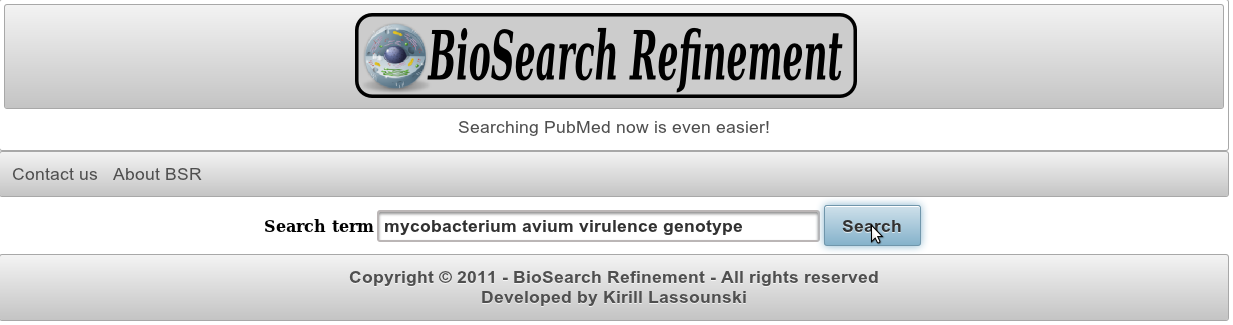
\includegraphics[scale=0.37]{imagens/telaInicial.png}
    \caption{Tela inicial do \emph{BioSearch Refinement} \label{fig:telaInicial}} 
\end{figure}

Na Figura \ref{fig:telaComBusca}, a aba foi aberta com o termo de busca solicitado e foram carregados os primeiros 20 artigos. Os artigos que são exibidos ficam guardados na memória (cacheados), se for feita a requisição para exibir outra página, e os artigos já exibidos ficam em \emph{cache} na sessão do navegador. Os artigos são exibidos em uma tabela similares à exibição do PubMed, informando o título, os autores, a revista na qual o trabalho foi publicado e o ano de publicação. Para visualizar informações complementares como o resumo do artigo, é necessário clicar na seta situada á esquerda para expandir um artigo.
\begin{figure}[h!]
    \center
    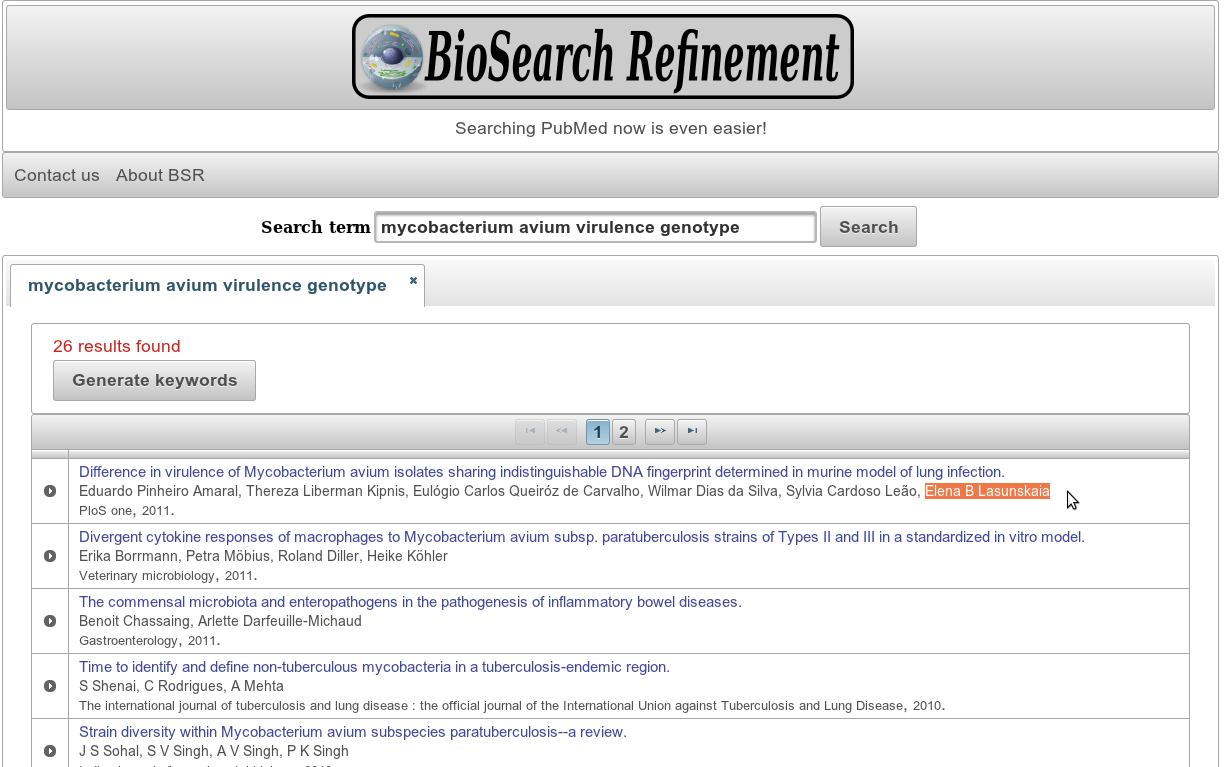
\includegraphics[scale=0.37]{imagens/telaComBusca.png}
    \caption{Tela após efetuar uma busca \label{fig:telaComBusca}} 
\end{figure}

Ao clicar no botão ''\emph{Generate keywords}'', o algoritmo \emph{Extraction Engine} é chamado para gerar as palavras-chave nos artigos que estão em \emph{cache}. Na Figura \ref{fig:palavrasChave} são mostradas as palavras-chave geradas para os artigos mostrados na figura anterior. Ao clicar em uma palavra-chave, uma nova aba será aberta. O título desta aba será o título da aba anterior concatenado com a palavra-chave selecionada, no exemplo da figura seria ''\emph{mycobacterium avium virulence genotype / mycobacterium avium subsp}''.

Existem dois tipos de abas no sistema, o primeiro se chama $LoadingTab$, esta aba representa o termo de busca inicial e implementa a paginação de artigos. A outra aba é a $OpenedTab$, gerada a partir de uma $LoadingTab$ e serve para mostrar os artigos refinados. Quando o usuário clica em uma palavra-chave, é aberta uma $OpenedTab$, e nesta aba as palavras-chave são recalculadas usando o \emph{Extraction Engine}. O processo de abertura de abas e processamento de palavras-chave é recursivo. 

As palavras-chave passam também por um processo de filtragem. Por exemplo, os termos que compõem o título da $LoadingTab$ da Figura \ref{fig:telaComBusca} (\emph{mycobacterium},\emph{avium},\emph{virulence},\emph{genotype}) são guardados em uma lista de \emph{stop words}. Se os termos da palavra-chave gerada pelo algoritmo \emph{Extraction Engine} estiverem na lista de \emph{stop words}, esta palavra-chave não será exibida, pois ela é irrelevante para o usuário. Ao abrir uma aba, a lista é incrementada com os termos da palavra-chave selecionada.

\begin{figure}[h!]
    \center
    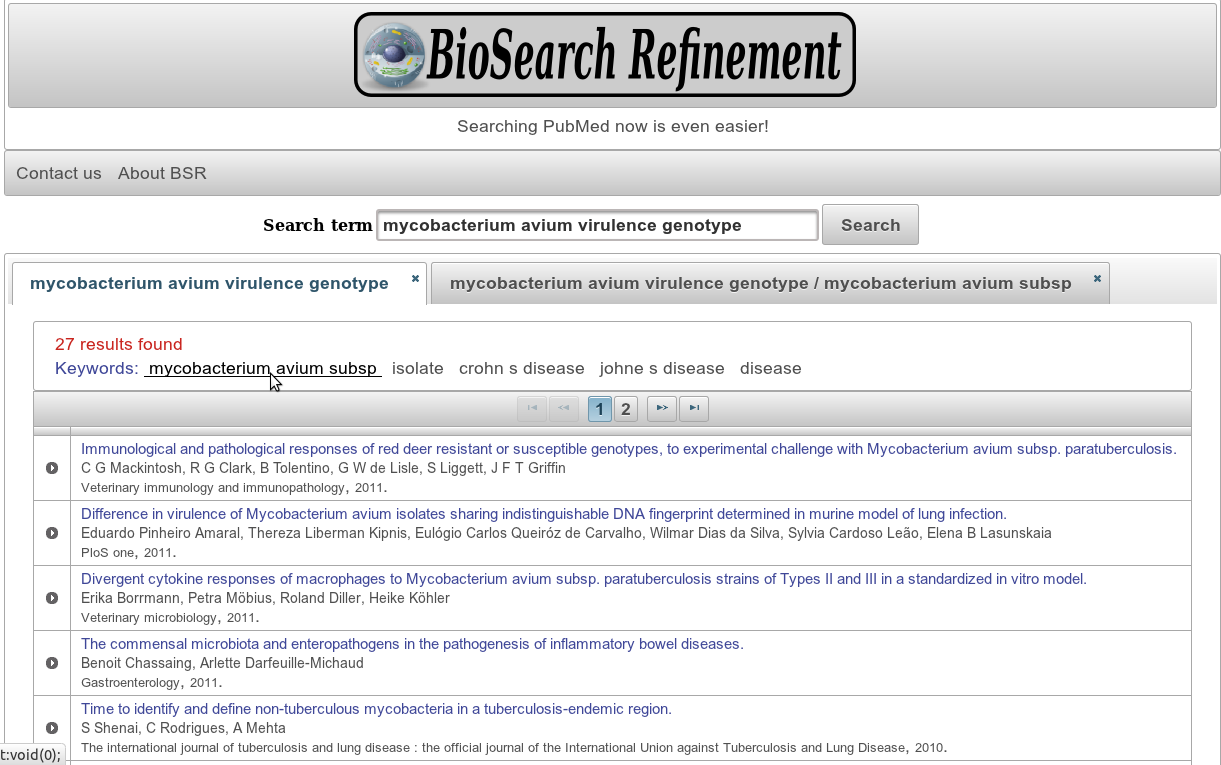
\includegraphics[scale=0.37]{imagens/telaComKwdsEAba.png}
    \caption{Palavras chave geradas pelo \emph{Extraction Engine} \label{fig:palavrasChave}} 
\end{figure}

\section{\emph{PubMed Dataset}}

Para avaliar o \emph{BioSearch Refinement} quanto à qualidade de suas predições e obter estatísticas importantes sobre os artigos do PubMed, é necessário um conjunto de programas que possibilitem a gestão destas informações. O \emph{PubMed Dataset} é uma API desenvolvida para a criação de conjuntos de dados teste com os artigos do PubMed, e também, serve como ponto de acesso ao PubMed no sistema \emph{BioSearch Refinement}. 

O objetivo principal do \emph{PubMed Dataset} é oferecer ao programador de um sistema de recuperação de informação o acesso aos dados do PubMed através do E-Utils \cite{Eutils2010} e a capacidade de gravar e ler estes dados do disco através de um programa Java. Isto é feito através de conjuntos de dados (\emph{datasets}) que são salvos em disco através de serialização (persistência de objetos). Um conjunto de dados é constituído de artigos científicos que são recuperados do PubMed utilizando um termo de busca, número máximo de artigos a serem recuperados e uma configuração de \emph{download}.

\subsection{E-Utils}
O E-Utils é um \emph{Web Service} composto por um conjunto de programas que utilizam URL`s (\emph{Uniform Resource Locator}) para fazer requisições e retornam dados em diversos formatos com HTML ou XML. Dentre estes programas, existem o E-Search, utilizado para fazer buscas, e o E-Fetch para recuperar os dados. O arquivo estruturado no formato XML do PubMed atende o padrão DTD (\emph{Document Type Definition}) do NLM Journal Archiving and Interchange, disponibilizado pelo NLM. O objetivo foi fornecer um formato comum que permitisse o intercâmbio de informação. Foram criados vários elementos, cada um com um propósito. Mas vale ressaltar que nem todos os artigos possuem todos os elementos, fato que deve cuidadosamente tratado com mecanismo de exceções. Dentro do arquivo XML estão os seguintes elementos:

\begin{itemize}
    \item <PMID> (PubMed ID): identificador único de um artigo
    \item <Article>:  é o elemento que contém os elementos que constituem um artigo.
    \item <ArticleTitle>:  título de um artigo.
    \item <Abstract>:  resumo de um artigo.
    \item <KeywordList>:  elemento que contém conjuntos de palavras-chave associadas com todo o documento e que podem ser usadas para fins de identificação e indexação. Estas palavras chave são atribuídas pelos autores do artigo.
    \item <MeshHeadingList>: lista de termos MeSH.
\end{itemize}
Estas informações são usadas pelo sistema \emph{BioSearch Refinement} para determinar as palavras-chave e exibir o conteúdo dos artigos. Além destes elementos, existem muitos outros que podem ser encontrados no DTD citado acima.

\subsection{Funcionalidades}
A Figura \ref{fig:processoGeralPMD} apresenta o funcionamento geral do PubMed Dataset que aparece na Figura \ref{fig:1}. A partir de parâmetros de entradas especificados, um termo de busca e um número máximo de artigos a ser recuperados, a ferramenta se conecta à base de dados PubMed através da internet. O processo de obtenção do conjunto de dados envolve os seguintes passos:
\begin{enumerate}
    \item Download de PMID`s: obtém os identificadores dos artigos que representam a busca efetuada pelo usuário utilizando o E-Search.
    \item Download de artigos: utilizando-se dos PMID`s, os artigos são recuperados em formato XML pelo E-Fetch.
    \item Extração dos atributos: através do processamento do documento XML, que é retornado do PubMed, são extraídos os atributos especificados na configuração de \emph{download} ($DownloadConfiguration$).
\end{enumerate}

\begin{figure}[h!]
    \center    
    \includegraphics[scale=0.5]{imagens/processoGeralPMD.pdf}
    \caption{Processo de obtenção de artigos do \emph{PubMed Dataset}\label{fig:processoGeralPMD}}
\end{figure}

Os parâmetros de entrada obrigatórios são:
\begin{itemize}
    \item o termo de busca que será utilizado para fazer uma query no banco de dados do
PubMed e que irá retornar um conjunto de artigos;
    \item número máximo de artigos a serem recuperados;
    \item os atributos que serão extraídos e usados para a criação das instâncias de um artigo. Se um dos atributos não for encontrado em um artigo contido no XML, este artigo será descartado. Como atributo de saída pode ser especificado qualquer elemento folha presente no arquivo XML.
\end{itemize}

O arquivo de saída é um arquivo serializado no formato ( ``\emph{termo de busca\_número de artigos\_articles.ser}'', ex: ``\emph{mycobacterium tuberculosis\_2754\_articles.ser}''). Este arquivo pode ser desserializado a qualquer momento e os artigos contidos neste estarão disponíveis prontamente. O diagrama de classes UML da biblioteca é apresentado na Figura \ref{fig:pubMedDatasetUML}.

\begin{landscape}
\begin{figure}[h!]
    \center    
    \includegraphics[scale=0.35]{imagens/pubMedDatasetUML.pdf}
    \caption{Diagrama de classes UML do \emph{PubMed Dataset} \label{fig:pubMedDatasetUML}}
\end{figure}
\end{landscape}

O  $ArticleDownloader$ é a classe responsável por obter os artigos do banco de dados PubMed e é construída com uma configuração $DownloadConfiguration$, que é onde são definidas as configurações do download. Nela são especificados os atributos que estarão presentes em cada artigo recuperado.

\begin{lstlisting}
DownloadConfiguration config = new DownloadConfiguration(ABSTRACT,AUTHOR,TITLE);
\end{lstlisting}

 Se o número máximo de artigos solicitados for muito grande, o processo de obtenção de artigos é fracionado em partes para evitar \emph{time out} por parte do servidor, isto é implementado no método $getDynaArticles()$ de $ArticleDownloader$. Primeiramente são obtidos os $PMID$’s através do E-Search e em seguida, utilizando estes, os artigos são recuperados e colocados em um DOM (\emph{Document Object Model}) utilizando o E-Fetch. O DOM é uma convenção para representar documentos XML e outros dentro de uma linguagem de programação. Em seguida, os elementos são percorridos e são
recuperados aqueles que foram selecionados pelo usuário no $DownloadConfiguration$.

Ao receber um $DownloadConfiguration$ o $ArticleDownloader$ pode efetuar a recuperação dos artigos através do método $getDynaArticles(termoDeBusca, maxHits)$ ou $getDynaArticles(termoDeBusca, primeiroArtigo, tamanhoDePagina)$. O primeiro método recebe um termo de busca, e o numero máximo de artigos que serão buscados no banco. O segundo método recupera uma fração de documentos, através dos dois últimos argumentos e pode ser usado para paginação. Ambos métodos retornam uma $List<DynaArticle>$ que possui as instâncias dos artigos que foram recuperados.

\begin{itemize}
\item $DynaArticle$ – Esta classe representa um artigo do PubMed. Possui uma
$Collection<Object>$ que serve para armazenar as palavras-chave geradas por um
algoritmo qualquer, e possui um $Map<String, ArticleAttribute>$ que serve para
guardar os atributos extraídos do PubMed. Um ponto importante é que esta classe por
possuir esta estrutura característica, permite que sejam criadas instâncias de artigos
dinamicamente, ou seja, com uma quantidade variável de atributos.

\item $ArticleAttribute$ – O atributo de um artigo é um dos fatores que permite a criação de
artigos dinâmicos. Esta classe possui nome do atributo, tipo do atributo e seu valor.

\end{itemize}
O $Dataset$ é quem vai encapsular os artigos e que será utilizado como unidade de persistência,
ou seja, será gravado em disco utilizando serialização. Mas esta classe nunca será utilizada
diretamente, pois possui um método abstrato chamado $generateKeyWords()$ que será
utilizado para o processo de geração de palavras-chave. Então, a utilização correta de um
$Dataset$ é se estendendo ele e implementando o método $generateKeyWords()$.

Como dito anteriormente, alguns artigos no PubMed podem não possuir determinados atributos, por isso o $ArticleDownloader$ possui uma variável booleana chamada $mandatoryAttributes$. Se o valor da variável for setado como \emph{true}, todos os atributos que foram passados na $DownloadConfiguration$ serão considerados obrigatórios, e os artigos que não possuírem algum destes atributos serão descartados.

Finalmente, a classe $DatasetSerializer$ é que faz a serialização e desserialização dos
$Dataset$`s. Na serialização, ela recebe o $Dataset$ a ser salvo em disco e um nome para o
arquivo que será salvo, geralmente um bom nome é o termo utilizado na criação do $Dataset$. A
este nome é acoplado o número de artigos existentes no $Dataset$ e a extensão “.ser” é
concatenada automaticamente. A desserialização é o processo inverso, no qual a partir do nome
de arquivo, o $Dataset$ é carregado para uma instancia.
É importante observar que quando o $Dataset$ é muito grande, pode ocorrer um erro de
\emph{java.lang.OutOfMemoryError: Java heap space}, pois a memória da máquina virtual Java
estoura e não consegue terminar a serialização ou o processo inverso. Para solucionar este
problema, a memória da maquina virtual deve ser aumentada, passando um parâmetro na linha
de comando:

\begin{lstlisting}
$ java -Xmx=256M seuProgramaQueEstouraAMemória
\end{lstlisting}

\section{\emph{Extraction Engine}}
O algoritmo \emph{Extraction Engine} foi desenvolvido como parte do sistema \emph{BioSearch Refinement} e é o componente do sistema que faz a extração das palavras-chave dos artigos e os organiza em tópicos mais abordados. A API de processamento de linguagem natural escolhida foi a \textbf{Alias-i Ling Pipe} que possui licença de uso gratuita para propósitos de pesquisa. Na recuperação e indexação dos artigos as palavras-chave jogam um papel integral, a extração de palavras-chave do corpo de um artigo tenta capturar a essência do assunto do mesmo, sem trabalhar com anotações humanas. A extração de palavras-chave é executada sobre os resumos dos artigos, pois a maioria dos artigos não disponibiliza o texto completo, mas apenas o resumo \cite{Hulth2003}.

A Figura \ref{fig:processoGeralEE} apresenta o esquema geral do algoritmo proposto para a obtenção das palavras-chave e a Figura \ref{fig:fluxoExecucaoEE} destaca um fluxo de execução para a obtenção de palavras-chave em um artigo. O algoritmo é dividido em vários passos, explicados a seguir. Para cada resumo:
\begin{figure}[h!]
    \center
    \includegraphics[scale=0.65]{imagens/processoGeralEE.pdf}
    \caption{Processo geral do algoritmo \emph{Extraction Engine} \label{fig:processoGeralEE}}
\end{figure}
\begin{figure}[h!]
    \center
    \includegraphics[scale=0.4]{imagens/fluxoExecucaoEE.pdf}
    \caption{Exemplo de obtenção de palavras-chave para um artigo \label{fig:fluxoExecucaoEE}}
\end{figure}
\begin{enumerate}
    \item \textbf{Divisão dos resumos em frases}: o texto de um resumo é composto por frases, um tokenizador trunca o texto em frases para utilizar na próxima etapa.

    \item \textbf{Rotulação ou POST (\emph{Part Of Speech Tagging})}: determina as classes gramaticais (\emph{tags}) de cada palavra na frase.

    \item \textbf{\emph{Noun Chunking}}: baseado no princípio de que os substantivos são os melhores descritores, o algoritmo seleciona termos compostos obrigatoriamente por substantivos. Para isto, foram definidos padrões sintáticos compostos por advérbios, adjetivos, numerais e alguns símbolos para conectar substantivos e formar termos mais descritivos.

    \item \textbf{Obtenção e seleção dos conceitos}: os conceitos servem para capturar a essência dos documentos e agrupar diversos \emph{noun chunks} similares em uma estrutura única. Um conceito é composto pelas palavras substantivas que compõem um \emph{chunk}, assim os termos \emph{green cells} e \emph{blue cells} fariam parte de um mesmo conceito \emph{cells}. São usados apenas os substantivos, pois o objetivo é generalizar o assunto sendo abordado no texto e agrupar assuntos semelhantes em um único conceito.

Para ilustrar a necessidade do uso de conceitos, observe os seguintes termos extraídos de um dos resumos: “\emph{other vegetable system}”, “\emph{the vegetable systems}” e “\emph{the vegetables}”. Se analisarmos as duas primeiras frases percebemos que elas tratam de um mesmo assunto “\emph{vegetable systems}”, porém a máquina irá tratar “\emph{system}”  e “\emph{systems}”  como duas palavras diferentes. Para contornar este tipo de discrepância é utilizado um algoritmo de normalização (\emph{stemming}). Usamos uma implementação do algoritmo de Porter \cite{Porter1980} fornecida pela API LingPipe, que permite remover sufixos de palavras em inglês.

Visto que as palavras são normalizadas, as frases “\emph{other vegetable system}” e “\emph{the vegetable systems}” são tratadas como sendo um mesmo conceito. Por outro lado, a terceira palavra só possui “\emph{vegetable}” como substantivo, o que acarreta na criação de um segundo conceito “\emph{vegetable}”.
\end{enumerate}



\subsection{Obtenção de conceitos}
O processo de conceitualização se divide em duas etapas. Na primeira etapa (conceitualização local), os conceitos são extraídos para cada artigo e são determinados os mais relevantes. Na segunda etapa (conceitualização global), são selecionados os conceitos que abordam a maior quantidade de artigos diferentes, determinando assim os temas mais abordados pelos artigos.

\subsubsection{Conceitualização local}
O processo de conceitualização se inicia com a criação de uma estrutura de armazenamento de conceitos, mostrada na Figura \ref{fig:conceitualizacaoLocalUML} chamada $ArticleConcepts$, que irá conter os conceitos de um determinado artigo. Um conceito é composto por um ou mais termos e cada um destes termos possui uma frequência no texto e pode possuir variações no texto como por exemplo plurais. Por isso um $Concept$ é composto por diversas partes $ConceptPart$, onde cada parte possui:
\begin{itemize}
    \item Peso ($weight$): representa a interação das partes de outros conceitos com este conceito, um processo de cruzamento de informações explicado adiante.
    \item Raiz da parte ($partStem$): a raiz da palavra que compõe esta parte para a comparação com outras partes.
    \item Mapa de frequência de ocorrência ($partWords$): usado para contar as frequências das diferentes palavras que em algum momento fizeram parte deste conceito.
\end{itemize}

\begin{figure}[h!]
    \center
    \includegraphics[scale=0.4]{imagens/conceitualizacaoLocalUML.pdf}
    \caption{Diagrama de classes de conceitualização local \label{fig:conceitualizacaoLocalUML}}
\end{figure}

Ao se criar um conceito, automaticamente, são criadas suas $ConceptPart$ e este conceito é adicionado em $ArticleConcepts$. Termos iguais ou similares são agrupadas sob o mesmo conceito. Por exemplo: o conceito “\emph{other vegetable system}” possui três partes: “$other$”, “$vegetable$” e “$system$”.  Ao aparecer “\emph{the vegetable systems}”, os conceitos seriam integrados utilizando a estrutura a seguir. A comparação entre os termos é feita na raiz de suas partes substantivas.

\textbf{Conceito: \emph{vegetable system}}

Parte 1 - Raiz: $vegetabl$, Mapa: $vegetable$ (frequência: 2)

Parte 2 - Raiz: $system$, Mapa: $system$ (frequência: 1), $systems$ (frequência: 1)

\subsubsection{Cruzamento de informações}
Para melhor descrever um artigo, é necessário avaliar cada conceito, valorizando os conceitos realmente relevantes e diminuindo o peso de conceitos pouco relevantes.

O processo de atribuição de peso de um conceito localmente é feito através um cruzamento de informação das partes de todos os conceitos similares a ele. Isso faz com que conceitos diferentes e com partes em comum recebam um peso maior, evidenciando ,assim, o grupo de conceitos que são mais abordados naquele artigo. Um conceito é similar a outro conceito, se estes possuem pelo menos uma parte em comum. A similaridade é calculada através da distância entre conceitos, e é a divisão do número de partes em comum pelo número de partes total do maior conceito.

A similaridade entre o $Conceito 1$ do exemplo anterior e o $Conceito 2$, a seguir, é calculado como: 

\begin{center}
\textbf{
similaridade = (núm. de partes em comum) / (núm. de partes do maior conceito)
}
\end{center}

\textbf{
\\ Conceito 1: \emph{vegetable systems}} \\
\textbf{
Conceito 2: \emph{vegetable oil}} \\
Partes em comum: 1 \\
Número de partes do maior conceito: 2 \\
Distância: ½ \\

O cruzamento de dois conceitos é feito para determinar o peso das partes similares, mostrado na Listagem \ref{lst:cruzamento}:
\lstset{caption={Cruzamento de dois conceitos},label=lst:cruzamento}
\begin{lstlisting}
    double weight = (fromPart.getPartFrequency() * distance);
    weight += toPart.getWeight();
    toPart.setWeight(weight);
\end{lstlisting}

Quanto maior a distância entre os conceitos, menor a influência de um no outro. O peso é atualizado para ambos os conceitos. Ao finalizar este processo, é feito o cálculo do peso dos conceitos utilizando-se do peso de suas partes, da frequência das partes e do número de partes que o conceito possui. O peso de um conceito é:

\(
\left(\sum_{partes}\medspace parte.frequencia + parte.peso\right) * \left(1 + fator\medspace de\medspace ajuste * num.\medspace de\medspace partes\right)
\)

Em primeiro lugar, é calculada a importância do conceito no texto do resumo. Para todas as partes de um conceito, é feito o somatório da sua frequência no texto e da sua interação com outros conceitos similares (peso do conceito). Este valor é então multiplicado pelo segundo parenteses da equação, onde é dada prioridade aos conceitos que possuem mais partes. Conceitos com mais partes são mais representativos, logo mais importantes. Além de aumentar a representatividade dos conceitos é feito o balanceamento entre a pequena quantidade de conceitos com muitas partes e pouca frequência e de conceitos com poucas partes e frequência alta. O fator de ajuste foi considerado 0.05 para que a cada parte que o conceito possui, ele receba um aumento no seu peso de 5\%, logo em um conceito de 4 partes este aumento é de 20\%. O valor do fator de ajuste foi determinado empiricamente.

Ao fim do processo, conceitos de apenas uma palavra e com menos de 4 letras são removidos, considerados pouco representativos.
Os conceitos com o maior peso são aqueles que foram mais referenciados no resumo, logo, são os melhores descritores. Cada conceito obtido pelo algoritmo é linearmente mapeado em uma predição de palavra-chave do artigo. Este processo é repetido para todos os resumos.

\subsubsection{Conceitualização global}

O processo de obtenção de conceitos é realizado em cada resumo de artigo. O conceito que referencia o maior número de artigos distintos tem maior importância, pois ele trata de um assunto comum, ou seja, é mais abordado em todos os artigos e passa a formar parte das palavras-chave globais. As palavras-chave globais formam o melhor conjunto de descritores para todos os artigos recuperados em uma consulta.

Cada conjunto de conceitos local é ordenado pelo peso decrescentemente, e deste conjunto apenas uma parte é selecionada para a conceitualização global. O principal motivo deste corte é a exclusão de conceitos pouco descritivos ou muito gerais que possuem pontuação relativamente baixa, e em segundo lugar a melhora da performance do sistema através da diminuição de conceitos a serem processados na fase global.

Resumos com maior quantidade de texto possuem mais palavras-chave do que resumos com algumas linhas, por isso a quantidade de conceitos selecionada é uma porcentagem do total de conceitos extraídos de um resumo. Foi verificado através de testes que os melhores resultados eram obtidos com a seleção de 35\% dos conceitos, assim eliminando 65\%.

No processo de globalização, os conceitos locais passam por uma verificação de integração, que permite que um mesmo conceito extraído de vários artigos seja unificado em um só. A unificação de conceitos implica na atualização da frequência desse conceito. Após a análise de todos os conceitos de todos os artigos, é feita a ordenação decrescente, seguindo os critérios: frequência (número de artigos que o referenciam) e peso do conceito. Os conceitos que possuem o maior número de artigos sendo referenciados, são os conceitos com maior abrangência, logo são considerados as melhores palavras-chave para sumarização.

Na \emph{interface} são exibidas as cinco melhores predições, mas algumas podem ser descartadas pelo algoritmo por serem consideradas como \emph{stop words}.

\subsection{Implementação}
Na Figura \ref{fig:conceitualizacaoUML} está representado o diagrama de classes do \emph{Extraction Engine}.
A classe que faz o processamento dos artigos é a $KeyWordProcessor$, ela também dá acesso aos conceitos mais referenciados através de um $Iterator<Concept>$ pelo método $getConceptIt()$. O método $processArticles$ recebe os artigos a serem processados e chama $conceptualize$. Este método irá percorrer todos os artigos, recuperar os resumos de cada um deles e tokenizá-los em frases usando o $SentenceSplitter$.

\begin{figure}[h!]
    \center
    \includegraphics[scale=0.25]{imagens/conceitualizacaoUML.pdf}
    \caption{Diagrama de classes de conceitualização\label{fig:conceitualizacaoUML}}
\end{figure}

As frases são passadas para o $MedLineSentenceChunker$ que determina os $TaggedChunk$`s de cada frase. Estes \emph{chunks} são usados na conceitualização local explicada anteriormente para determinar os conceitos mais relevantes de um artigo.

Os conceitos obtidos localmente são guardados no $GlobalConceptHolder$ através do método $insertConcept$. A cada conceito que é inserido, é feita uma busca para determinar se um conceito parecido conceitualmente já existe. A comparação de dois conceitos é feita através de uma chave, que é composta pelas raízes das partes de um conceito. Se dois conceitos são similares, a lista de PMID`s deste conceito é incrementada como também a frequência de ocorrência de suas partes.

Após todos os conceitos serem inseridos no $GlobalConceptHolder$, é chamado o método $sortConcepts$ para que os conceitos sejam ordenados segundo o seu número de PMID`s e depois por frequência de ocorrência. Nesta etapa o \emph{BioSearch Refinement} já pode obter o $Iterator<Concept>$ para navegar pelos conceitos mais referenciados e selecionar as palavras-chave.

    \chapter{Resultados}

Neste capítulo são apresentados os resultados para a biblioteca \emph{PubMed Dataset}, o algoritmo de sumarização \emph{Extraction Engine} e o sistema \emph{BioSearch Refinement}. Os dados utilizados na analise do \emph{PubMed Dataset}, foram utilizados para avaliar o \emph{Extraction Engine} com uma perspectiva diferente.

\section{Resultados do \emph{PubMed Dataset}}
Para a criação dos conjuntos de dados primeiramente foram definidos os termos de busca, o
número máximo de artigos a ser buscado e em seguida foram definidos os atributos dos artigos
que seriam necessários nos conjunto de dados. Cada artigo necessita conter o resumo que será
utilizado para a obtenção das palavras chave geradas pelo algoritmo e também das palavras
chave definidas pelos autores, pois estas são a referência da comparação com as palavras
automaticamente extraídas pelo \emph{Extraction Engine}.

Existem dois tipos de palavras-chave usadas na base de dados do PubMed: os termos de
indexação MeSH e as palavras-chave fornecidas pelos autores do artigo. Os experimentos foram
realizados utilizando como referência os termos MeSH, pois se encontraram poucos artigos com
palavras-chave dos autores.

A biblioteca foi avaliada sob os seguintes aspectos: facilidade de uso (linhas de código para executar a tarefa desejada) e performance (tempo de execução). O objeto de estudo foi a criação de dois conjuntos de dados que seriam utilizados para analisar o \emph{Extraction Engine}, mostrados na Tabela \ref{tab:datasets}.


\begin{table}[htbp]
\center
\begin{tabular}{|l|l|}
\hline
\multicolumn{ 2}{|c|}{\textbf{Conjunto de dados 1}} \\ \hline
Termo de busca & \textit{mycobacterium tuberculosis} \\ \hline
Número de artigos solicitados & \multicolumn{1}{r|}{10000} \\ \hline
Número de artigos recuperados & \multicolumn{1}{r|}{8045} \\ \hline
\multicolumn{ 2}{|c|}{\textbf{Conjunto de dados 2}} \\ \hline
Termo de busca & \textit{h1n1 influenza virus} \\ \hline
Número de artigos solicitados & \multicolumn{1}{r|}{5000} \\ \hline
Número de artigos recuperados & \multicolumn{1}{r|}{2858} \\ \hline
\end{tabular}
\caption{Conjuntos de dados criado com o PubMed Dataset}
\label{tab:datasets}
\end{table}

Para a criação de um conjunto de dados (\emph{dataset}), são necessárias no mínimo 5 linhas de código. O método da Listagem \ref{lst:datasetCreation} recebe o termo de busca e o número de artigos a ser buscado, em seguida, é criada a configuração de \emph{download} com os atributos necessários e o $ArticleDownloader$ com esta configuração. Os atributos são configurados como obrigatórios, ou seja, todos os artigos devem possuir os atributos solicitados e então é feito o \emph{download} dos artigos. Finalmente os artigos são passados para o serializador que os salva em disco com o nome do termo para identificação.

\lstset{caption={Criação de um \emph{DataSet}},label=lst:datasetCreation}
\begin{lstlisting}
public void criarDataSet(String termo, int quantidade) throws IOException{
    DownloadConfiguration config = new DownloadConfiguration(PMID,ABSTRACT,MESH_TERMS);
    ArticleDownloader downloader = new ArticleDownloader(config);
    downloader.setMandatoryAttributes(true);
    List<DynaArticle> downloadedArticles = downloader.getDynaArticles(termo, quantidade);
    DataSet conceptDS = new ConceptDataSet(articles, "mycobacterium tuberculosis");
    DataSetSerializer.serializeDataSet(conceptDS, termo);
}
\end{lstlisting}

Após a criação dos conjuntos de dados, foram executadas duas rotinas implementadas na classe $ConceptDataSet$ que estende $DataSet$. A primeira ($removeSearchTermFromData()$), remove o termo de busca dos conjuntos de palavras-chave geradas e termos MeSH, pois são irrelevantes para o pesquisador já que ele as usou como termo de busca. A segunda rotina ($intersectKws_Abstract$) desconsidera os termos MeSH que não estão no texto do resumo, pois como o algoritmo avaliado é de extração, só se pode comparar palavras chave extraídas com palavras do próprio resumo.

Como pode-se perceber, a quantidade de artigos recuperados difere da quantidade solicitada. Alguns dos motivos que causaram a redução do número de artigos nos conjuntos de dados foram: alguns artigos no PubMed não possuem os atributos solicitados na configuração de \emph{download}. As rotinas descritas no parágrafo acima causam a exclusão de alguns artigos, quando estes ficam sem palavras-chave geradas ou termos MeSH.

\subsection{Discussão dos resultados do \emph{PubMed Dataset}}

Com a utilização da ferramenta, a construção dos conjuntos de dados aconteceu de maneira
rápida e fácil, bastando apenas especificar os parâmetros iniciais. A utilização do conjunto de
dados se torna muito flexível, pois os seus dados podem ser alterados e gravados novamente,
seja para atualizar as palavras-chave geradas ou algum outro parâmetro.

A partir da Tabela \ref{tab:tempoExecucao}, pode-se observar que, apesar do tempo para download ter sido
consideravelmente grande para 10.000 artigos, esta fase só é executada uma vez, pois o
conjunto de dados é gravado em disco após a execução e sempre vai ser dependente do tráfego
na rede. Pode-se ver que o tempo levado para carregar o conjunto de dados é muito pequeno,
tornando sua utilização muito conveniente para testes. A quantidade de artigos recuperados
varia muito de acordo com os atributos que foram especificados pelo usuário, quanto maior o
numero destes, menos artigos serão recuperados, pois menor será a probabilidade de um artigo
possuir todos os atributos solicitados. A qualidade dos dados recuperados dependerá do que for
disponibilizado no PubMed, pois os conjuntos de dados criados são uma reflexão dos dados
contidos no banco de dados de origem.

\begin{table}[htbp]
\center
\begin{tabular}{|l|l|l|}
\hline
\textbf{Conjunto de dados} & \textbf{Etapas} & \textbf{Tempo de execução} \\ \hline
\multicolumn{ 1}{|c|}{\textbf{1}} & \textit{Download} & 7,45 minutos \\ \cline{ 2- 3}
\multicolumn{ 1}{|l|}{} & Serialização & 2 segundos \\ \cline{ 2- 3}
\multicolumn{ 1}{|l|}{} & Desserialização & 3 segundos \\ \hline
\multicolumn{ 1}{|c|}{\textbf{2}} & \textit{Download} & 3,11 minutos \\ \cline{ 2- 3}
\multicolumn{ 1}{|l|}{} & Serialização & 859 milissegundos \\ \cline{ 2- 3}
\multicolumn{ 1}{|l|}{} & Desserialização & 1 segundo \\ \hline
\end{tabular}
\caption{Desempenho da ferramenta PubMed Dataset na construção dos conjuntos de dados}
\label{tab:tempoExecucao}
\end{table}

Em um ambiente de teste e avaliação, os testes são criados progressivamente e muitas vezes são adicionados casos de teste mais específicos. Dado esse cenário, é óbvio o fato de que os testes são executados diversas vezes. Sem a utilização desta biblioteca, o tempo gasto para a criação dos dados de teste e execução dos testes propriamente ditos levariam um tempo
considerável. Como podemos observar na Tabela \ref{tab:tempoExecucao}, o tempo gasto para o download dos dados é muito grande e também devemos ressaltar que a consistência do conjunto de dados não é garantida visto que os dados retornados pelo PubMed podem variar com o passar do tempo.

\section{Resultados do \emph{Extraction Engine}}

O ponto crucial do \emph{Extraction Engine} é extrair descritores válidos para cada artigo, pois se os descritores selecionados localmente são de qualidade, a sumarização dos artigos no processo global será eficiente. 


    \chapter{Conclusões}

Todos os objetivos definidos no início do projeto foram atingidos, resultando em um sistema funcional e eficiente. A seguir são dadas as conclusões finais sobre o sistema e suas partes, como também, são apresentadas as contribuições e trabalhos futuros.

\section{\emph{PubMed Dataset}}
O \emph{PubMed Dataset} se mostrou uma ótima ferramenta para a criação de conjunto de dados de teste, facilitando em grande parte o processo de avaliação do algoritmo de extração. O módulo de \emph{download} que realiza a conexão com os servidores do NCBI foi projetado de maneira que seja flexível, possibilitando a adição de novos parâmetros com algumas linhas de código.

O tempo levado para carregar e escrever os \emph{datasets} para a memória é de alguns segundos, sendo muito útil em baterias de teste. Já o tempo levado para obter os artigos depende de diversos fatores independentes da biblioteca, como condição de carga do banco de dados do PubMed e velocidade de conexão do usuário.

Por ser código aberto, pode ser aprimorado pela comunidade de bioinformática para ser uma biblioteca ainda mais funcional. O projeto se encontra no repositório Git do GitHub no endereço \url{https://github.com/lassounski/PubMed-Dataset} ou em formato .jar no repositório Maven. A dependência e o repositório que devem ser adicionados podem ser vistos nas Listagens 3 e 4.
\lstset{caption={Dependência Maven},label=lst:pmdDependecy}
\begin{lstlisting}
<dependency>
    <groupId>com.uenf</groupId>
    <artifactId>PubMedDataset</artifactId>
    <version>1.0-SNAPSHOT</version>
</dependency>
\end{lstlisting}
\lstset{caption={Repositório Maven},label=lst:pmdRepository}
\begin{lstlisting}
<repository>
    <id>lassounski-snapshots</id>
    <url>https://github.com/lassounski/mvn-repo/raw/master/snapshots</url>
</repository>
\end{lstlisting}

A utilização do \emph{PubMed Dataset} no \emph{BioSearch Refinement} se mostrou muito útil, já que os artigos exibidos no sistema são obtidos usando a ferramenta. O tempo levado pela aplicação para exibir as páginas de artigos é aceitável, sendo um pouco maior do que o tempo levado pelo próprio NCBI.

\section{\emph{Extraction Engine}}

O algoritmo de extração de palavras-chave obteve bons resultados possuindo um \emph{recall} em torno de 70\%, ou seja, dos termos MeSH atribuídos aos artigos que existem no texto, 70\% foram recuperados pelo algoritmo.

As palavras-chave exibidas para o usuário destacam os assuntos mais abordados pelos artigos e representam sub-conjuntos do original, que podem ajudar no processo de busca. Uma expansão no algoritmo poderia permitir que o usuário navegue pelas palavras-chave através de um modelo de hierarquia, onde palavras-chave mais gerais contem palavras-chave mais específicas.

Vale notar que o \emph{Extraction Engine} pode ser usado para outras áreas de aplicação diferentes da biomedicina. O que tem de ser modificado para que o algoritmo se adapte à uma determinada área de conhecimento é o seu \emph{part of speech tagger} que vai determinar as classes gramaticais das palavras.

\section{\emph{BioSearch Refinement}}

O sistema desenvolvido possui uma \emph{interface} enriquecida com componentes visuais animados que favorecem a usabilidade, a navegação por abas facilita a organização da informação do usuário. O tempo de resposta da aplicação é aceitável, mas pode ser melhorado com técnicas de otimização.

\section{Contribuições}
O resultado do trabalho desenvolvido é de código aberto e é disponibilizado para utilização e/ou modificação, melhoramentos podem ser submetidos para a origem e serão avaliadas. Tanto a biblioteca \emph{PubMed Dataset} como o sistema \emph{BioSearch Refinement} podem ser encontrados no GitHub em \url{https://github.com/lassounski/PubMed-Dataset} e \url{https://github.com/lassounski/BioSearch-Refinement}.

O \emph{PubMed Dataset} foi apresentado e publicado no BIOINFORMATICS 2012 (\emph{International Conference on Bioinformatics Models, Methods and Algorithms}). E o \emph{BioSearch Refinement} foi aceito para publicação na Conferência IADIS Ibero Americana de 2011.

\section{Trabalhos futuros}
As perspectivas de trabalhos futuros por parte do \emph{Extraction Engine} visam uma mudança na arquitetura do algoritmo para permitir a categorização de conceitos por hierarquias. Mesmo conceitos diferentes como "platelets flow",\ "platelet",\ "platelet plasma"\ e "platelets expression", possuem
 "platelet" \ como conceito mestre. Este conceito estaria na raiz da árvore como conceito pai e os outros conceitos seriam englobados nestes como filhos. Um determinado conceito poderia ser filho de n conceitos pais e poderia ter m filhos, a relevância de um conceito na árvore seria representada pelo seu número de partes, número de filhos e frequência de ocorrência das partes similares.
 

    \citeoption{abnt-repeated-author-omit=yes}
    \bibliographystyle{abnt-alf}
    \bibliography{bibliografia}

\end{document}

